

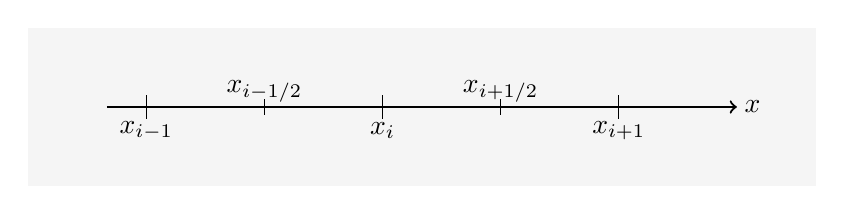
\begin{tikzpicture}
\draw[fill=gray!8,gray!8](0,0) rectangle (10,2);
%\draw[step=0.5cm,gray,very thin] (0,0) grid (8,5); %background grid


%\draw[fill=gray!13,gray!13](1,1) rectangle (8,3);
%\draw[thick] (1,1) -- (5,1) -- (5,4) -- (1,4) -- cycle;  

\draw[thick,->] (1,1) -- (9,1) ; 

\draw[-] (1.5,0.85) -- (1.5,1.15) ; 
\draw[-] (4.5,0.85) -- (4.5,1.15) ; 
\draw[-] (7.5,0.85) -- (7.5,1.15) ; 

\node[] at (1.5,0.7) {$x_{i-1}$};
\node[] at (4.5,0.7) {$x_i$};
\node[] at (7.5,0.7) {$x_{i+1}$};

\node[] at (3,1.2) {$x_{i-1/2}$};
\node[] at (6,1.2) {$x_{i+1/2}$};
\draw[-] (3,0.9) -- (3,1.1) ; 
\draw[-] (6,0.9) -- (6,1.1) ; 

\node[] at (9.2,1) {$x$};
\end{tikzpicture}
